\chapter{Mecánica de medios continuos y elasticidad}\label{ch:b3:continuum-elasticity}

Péguese el oído a un largo raíl de acero mientras un operario lo golpea a lo
lejos: oirá dos golpes --- uno por el acero y otro por el aire ---
separados por un segundo o más. La roca, el acero, el hueso y el caucho
transmiten fuerzas y ondas como un fluido transmite la presión, pero con
algo que ningún fluido tiene: se resisten a los \emph{cambios de forma}, y
no solo a los de volumen. El volumen del Año 2 construyó la mecánica de
fluidos sobre dos ideas, la partícula material y el campo de presión; este
capítulo las extiende a los sólidos. El desplazamiento de cada partícula
pasa a ser un campo, su distorsión local una \emph{deformación}, las fuerzas
internas una \emph{tensión}, y entre ambas se sitúa el carné de identidad
del sólido: la \omterm{thm:b3:continuum-elasticity:hooke}{ley de Hooke} con sus dos constantes elásticas. El provecho va
desde lo cotidiano --- por qué se alargan los cables, por qué revientan las
botellas, cómo se dobla un trampolín --- hasta lo planetario: los terremotos
envían a través de la Tierra exactamente las dos clases de onda elástica que
este capítulo predice, y sus tiempos de llegada fueron la primera escucha
del interior de nuestro planeta.

\section{La deformación: describir el cambio de forma}

\begin{definition}[Campo de desplazamientos y tensor de deformaciones]\label{def:b3:continuum-elasticity:strain}
\index{campo de desplazamientos}\index{tensor de deformaciones}\index{dilatación cúbica}
Cuando un sólido se deforma, la partícula que estaba inicialmente en
$\vect r$ pasa a $\vect r + \vect u(\vect r)$: $\vect u$ es el \emph{campo
de desplazamientos}. Para deformaciones pequeñas, la distorsión local se
mide con el \emph{tensor de deformaciones}, la matriz simétrica
\[
\varepsilon_{ij} = \frac12\Big(
 \frac{\partial u_i}{\partial x_j} + \frac{\partial u_j}{\partial x_i}
\Big) , \qquad i, j \in \{x, y, z\} .
\]
Una componente diagonal $\varepsilon_{xx}$ es el alargamiento relativo del
material en la dirección $x$ (adimensional; por ejemplo $\num{e-3}$ para un
cable de acero en servicio); una componente no diagonal $\varepsilon_{xy}$
es la mitad del cierre del ángulo entre las direcciones materiales $x$ e $y$
--- una \emph{cizalladura}. La traza es la variación relativa de volumen, la
\emph{dilatación cúbica}:
\[
\frac{\delta V}{V} = \varepsilon_{xx} + \varepsilon_{yy} +
\varepsilon_{zz} = \operatorname{div}\vect u .
\]
\end{definition}

\begin{example}[Tres deformaciones elementales]\label{ex:b3:continuum-elasticity:elementary}
Dilatación uniforme $\vect u = \alpha\vect r$: $\varepsilon_{ij} =
\alpha\,\delta_{ij}$, variación de volumen $3\alpha$, sin cizalladura.
Cizalladura simple $\vect u = (\gamma y, 0, 0)$: $\varepsilon_{xy} = \gamma/2$
y todas las componentes diagonales nulas --- la forma cambia, el volumen no.
Rotación rígida $\vect u = (-\omega y, \omega x, 0)$:
$\varepsilon_{ij} = 0$ idénticamente --- la parte antisimétrica de
$\partial u_i/\partial x_j$, que la simetrización descarta, es precisamente
la que gira sin deformar. La deformación mide solo el cambio de forma.
\end{example}

\begin{omfigure}
\begin{tikzpicture}[font=\small, >=Stealth]
  % stretch
  \begin{scope}
    \draw[gray, dashed] (0,0) rectangle (1.6,1.6);
    \draw[omDef, thick] (-0.2,0.16) rectangle (1.8,1.44);
    \draw[->] (2.0,0.8) -- (2.55,0.8);
    \draw[->] (-0.4,0.8) -- (-0.95,0.8);
    \node at (0.8,-0.85) {alargamiento $\varepsilon_{xx} > 0$,};
    \node at (0.8,-1.3) {contracción $\varepsilon_{yy} < 0$};
  \end{scope}
  % shear
  \begin{scope}[xshift=5.3cm]
    \draw[gray, dashed] (0,0) rectangle (1.6,1.6);
    \draw[omThm, thick] (0,0) -- (1.6,0) -- (2.0,1.6) -- (0.4,1.6) -- cycle;
    \draw[->] (0.9,1.8) -- (1.5,1.8);
    \draw[->] (0.7,-0.2) -- (0.1,-0.2);
    \node at (0.9,-0.85) {cizalladura $\varepsilon_{xy} = \gamma/2$:};
    \node at (0.9,-1.3) {cambia la forma, no el volumen};
  \end{scope}
  % rotation
  \begin{scope}[xshift=10.6cm]
    \draw[gray, dashed] (0,0) rectangle (1.6,1.6);
    \begin{scope}[rotate around={14:(0.8,0.8)}]
      \draw[omExo, thick] (0,0) rectangle (1.6,1.6);
    \end{scope}
    \draw[->] (1.75,1.5) arc (30:80:1.1);
    \node at (0.8,-0.85) {rotación: $\varepsilon_{ij} = 0$,};
    \node at (0.8,-1.3) {ninguna deformación};
  \end{scope}
\end{tikzpicture}

{\small El \omterm{def:b3:continuum-elasticity:strain}{tensor de deformaciones} solo ve la deformación verdadera:
el estiramiento (componentes diagonales), la cizalladura (componentes no
diagonales) --- y una rotación rígida, en absoluto.}
\end{omfigure}

\section{La tensión: describir las fuerzas internas}

\begin{definition}[Vector tensión y tensor de tensiones]\label{def:b3:continuum-elasticity:stress}
\index{tensor de tensiones}\index{vector tensión}
Córtese el sólido, mentalmente, a lo largo de una pequeña superficie $\dd S$
de normal $\vect n$: el material del lado $+\vect n$ tira del otro lado con
una fuerza $\dd\vect F = \boldsymbol\sigma(\vect n)\,\dd S$ --- el
\emph{vector tensión}. Esta fuerza depende linealmente de $\vect n$
(Cauchy), de modo que la codifica el \emph{tensor de tensiones}
$\sigma_{ij}$:
\[
\dd F_i = \sum_j \sigma_{ij}\,n_j\,\dd S ,
\]
en pascales. $\sigma_{xx}$ es una tracción ($> 0$) o una compresión ($< 0$)
a través de una cara normal a $x$; $\sigma_{xy}$ es una fuerza dirigida
según $x$ soportada por una cara normal a $y$ --- una tensión cortante. Un
fluido en reposo es el caso particular $\sigma_{ij} = -p\,\delta_{ij}$: la
presión empuja por igual sobre cada cara y no cizalla ninguna, y por eso los
fluidos fluyen --- no pueden soportar una cizalladura estática.
\end{definition}

\begin{proposition}[Equilibrio y simetría]\label{prop:b3:continuum-elasticity:equilibrium}
En un sólido en equilibrio bajo una fuerza másica $\vect f$ por unidad de
volumen (por ejemplo $\rho\vect g$),
\[
\sum_j\frac{\partial\sigma_{ij}}{\partial x_j} + f_i = 0
\]
en todo punto interior; y el \omterm{def:b3:continuum-elasticity:stress}{tensor de tensiones} es simétrico,
$\sigma_{ij} = \sigma_{ji}$.
\end{proposition}

\begin{proof}[Demostración parcial]
Equilibremos las fuerzas sobre un pequeño cubo de arista $a$: los \omterm{def:b3:continuum-elasticity:stress}{vectores
tensión} sobre las dos caras normales a $x$ difieren en
$a\,\partial_x\sigma_{ix}$ por unidad de área, y lo mismo para las demás
parejas; la fuerza superficial neta por unidad de volumen es
$\sum_j\partial_j\sigma_{ij}$, que debe cancelar $f_i$ --- la misma
contabilidad que dio $-\vect\nabla p + \rho\vect g = \vect 0$
en la estática de fluidos del volumen del Año 1. La simetría: el momento de
las tensiones cortantes respecto del centro del cubo es $(\sigma_{xy} -
\sigma_{yx})a^3$ en el orden dominante, mientras que su momento de inercia
va como $a^5$; una tensión asimétrica haría girar los cubos pequeños
infinitamente deprisa. El argumento continuo completo se admite.
\end{proof}

\begin{omfigure}
\begin{tikzpicture}[font=\small, >=Stealth, scale=1.05]
  % cube in light 3D
  \coordinate (A) at (0,0); \coordinate (B) at (2.4,0);
  \coordinate (C) at (2.4,2.4); \coordinate (D) at (0,2.4);
  \coordinate (E) at (0.9,0.75); \coordinate (F) at (3.3,0.75);
  \coordinate (G) at (3.3,3.15);
  \draw[thick] (A) -- (B) -- (C) -- (D) -- cycle;
  \draw[thick] (B) -- (F) -- (G) -- (C);
  \draw[thick] (D) -- (0.9,3.15) -- (G);
  \draw[thick, dashed] (A) -- (E) -- (F);
  \draw[thick, dashed] (E) -- (0.9,3.15);
  % normal stress on +x face
  \draw[->, omThm, very thick] (2.85,1.55) -- (4.05,1.55);
  \node[omThm, anchor=west] at (4.1,1.55) {$\sigma_{xx}$};
  % shear on +x face
  \draw[->, omDef, very thick] (2.85,1.9) -- (2.85,3.0);
  \node[omDef, anchor=south] at (2.85,3.05) {$\sigma_{yx}$};
  \draw[->, omExo, very thick] (3.1,1.3) -- (2.5,0.85);
  \node[omExo, anchor=east] at (2.35,0.48) {$\sigma_{zx}$};
  \node at (1.2,1.2) {cara $\perp x$};
  \node[align=left, anchor=west, font=\footnotesize] at (5.6,2.3)
    {$\sigma_{xx}$: tracción/compresión\\[2pt]
     $\sigma_{yx}$, $\sigma_{zx}$: tensiones cortantes\\[2pt]
     soportadas por la misma cara};
\end{tikzpicture}

{\small Las tres componentes del \omterm{def:b3:continuum-elasticity:stress}{vector tensión} sobre una cara de un cubo
material: una normal (tracción o compresión) y dos tangenciales
(cortantes). Las nueve componentes sobre las tres caras forman el \omterm{def:b3:continuum-elasticity:stress}{tensor de
tensiones}.}
\end{omfigure}

\section{La ley de Hooke y las constantes elásticas}

\begin{theorem}[Elasticidad lineal isótropa]\label{thm:b3:continuum-elasticity:hooke}
\index{ley de Hooke}\index{módulo de Young}\index{coeficiente de Poisson}
Para deformaciones pequeñas, un sólido isótropo responde linealmente: la
tensión es proporcional a la deformación,
\[
\sigma_{ij} = \lambda\,(\varepsilon_{xx} + \varepsilon_{yy} +
\varepsilon_{zz})\,\delta_{ij} + 2\mu\,\varepsilon_{ij} ,
\]
con dos constantes del material, los \emph{coeficientes de Lamé} $\lambda$ y
$\mu$ ($\mu$ se escribe también $G$, el \emph{módulo de cizalladura}). En el
ensayo de tracción simple --- una barra estirada según $x$ y libre por sus
costados --- la misma ley toma la forma del ingeniero
\[
\varepsilon_{xx} = \frac{\sigma_{xx}}{E} , \qquad
\varepsilon_{yy} = \varepsilon_{zz} = -\nu\,\varepsilon_{xx} ,
\]
que define el \emph{\omterm{thm:b3:continuum-elasticity:hooke}{módulo de Young}} $E$ (rigidez frente al estiramiento) y
el \emph{\omterm{thm:b3:continuum-elasticity:hooke}{coeficiente de Poisson}} $\nu$ (contracción lateral), con
\[
\mu = \frac{E}{2(1 + \nu)} , \qquad
\lambda = \frac{E\nu}{(1 + \nu)(1 - 2\nu)} .
\]
Es el ``cuanto el alargamiento, tanta la fuerza'' de Hooke (1678), elevado
a tensor. Vale hasta un \emph{límite elástico} propio de cada material.
\end{theorem}
\admitted

\begin{remark}[Órdenes de magnitud]\label{rem:b3:continuum-elasticity:orders}
$E \approx \qty{200}{GPa}$ para el acero, \qty{70}{GPa} para el aluminio y
el vidrio de ventana, \qty{50}{GPa} para el granito, \qty{15}{GPa} para el
hueso y el hormigón, \qty{10}{GPa} para la madera en la dirección de la
fibra y solo unos pocos MPa para el caucho --- cinco órdenes de magnitud,
la distancia entre un puente y una goma elástica. $\nu$ está comprendido
entre $0$ (el corcho, casi) y $1/2$ (el caucho): $\nu = 1/2$ significa
deformación a volumen constante, y $\nu \approx 0.3$ es lo típico de los
metales. Una deformación de $\num{e-3}$ en acero significa ya
$\sigma = \qty{200}{MPa}$, cerca del límite de fluencia de las calidades
ordinarias: la elasticidad cotidiana vive por debajo de una milésima.
\end{remark}

\begin{example}[El cable de un ascensor]\label{ex:b3:continuum-elasticity:cable}
Un cable de acero de \qty{60}{m} y sección \qty{2.0}{cm^2} sostiene una
cabina de \qty{1000}{kg}: $\sigma = mg/S = \qty{49}{MPa}$, $\varepsilon =
\sigma/E = \num{2.5e-4}$, alargamiento $\varepsilon L = \qty{15}{mm}$ ---
y el cable se comporta como un resorte de rigidez $k = ES/L =
\qty{6.7e5}{N/m}$: la fórmula $k = ES/L$ es la manera en que un medio
continuo devuelve los resortes del volumen del Año 1.
\end{example}

\begin{proposition}[Energía elástica]\label{prop:b3:continuum-elasticity:energy}
\index{energía elástica}
Un sólido deformado almacena, por unidad de volumen, la densidad de energía
\[
w = \frac12\sum_{i,j}\sigma_{ij}\,\varepsilon_{ij}
\qquad\text{(tracción simple: } w = \tfrac12 E\varepsilon^2 =
\sigma^2/2E\text{)} ,
\]
el $\tfrac12 kx^2$ tridimensional.
\end{proposition}

\begin{proof}[Demostración parcial]
En tracción simple, llevar la tensión de $0$ a $\sigma$ realiza el trabajo
por unidad de volumen $\int_0^\varepsilon\sigma'\,\dd\varepsilon' =
\int_0^\varepsilon E\varepsilon'\,\dd\varepsilon' = \tfrac12
E\varepsilon^2$ --- el área bajo la recta tensión--deformación, exactamente
como para un resorte. La forma cuadrática general se sigue superponiendo las
componentes; se admite.
\end{proof}

\begin{omfigure}
\begin{tikzpicture}[font=\small, >=Stealth]
  % traction test sketch
  \begin{scope}[yshift=0.4cm]
    \draw[gray, dashed] (0,0) rectangle (3.2,1.0);
    \draw[omDef, thick] (-0.25,0.07) rectangle (3.45,0.93);
    \draw[->, very thick] (3.65,0.5) -- (4.55,0.5) node[right] {$F$};
    \draw[->, very thick] (-0.45,0.5) -- (-1.35,0.5) node[left] {$F$};
    \draw[<->] (0,-0.35) -- (3.2,-0.35);
    \node at (1.6,-0.7) {$L(1 + \varepsilon)$};
    \node at (1.6,1.55) {sección $S$, $\sigma = F/S$};
  \end{scope}
  % stress-strain curve
  \begin{scope}[xshift=7.3cm, yshift=-0.6cm]
  \begin{axis}[omaxis, axis x line=bottom, axis y line=left,
    width=6.4cm, height=4.6cm, xmin=0, xmax=10, ymin=0, ymax=1.25,
    xlabel={$\varepsilon$}, ylabel={$\sigma$},
    xlabel style={at={(axis description cs:0.5,-0.1)}, anchor=north},
    xtick=\empty, ytick=\empty, clip=false]
    \addplot[omDef, very thick, domain=0:2] {0.4*x};
    \addplot[omExo, thick, domain=2:8.7, samples=40]
      {0.8 + 0.32*(1-exp(-(x-2)/2.2))};
    \fill (axis cs:2,0.8) circle (1.6pt);
    \draw (axis cs:2.05,0.83) -- (axis cs:2.55,1.1);
    \node[font=\scriptsize, anchor=west] at (axis cs:2.55,1.14) {límite elástico};
    \node[font=\scriptsize, omExo, anchor=west] at (axis cs:4.6,0.87) {flujo plástico};
    \node[font=\scriptsize, anchor=west] at (axis cs:8.55,1.2) {fractura};
    \fill[omThm] (axis cs:8.7,1.115) circle (1.6pt);
    \node[font=\scriptsize, omDef, rotate=38, anchor=south] at (axis cs:1.15,0.48) {pendiente $E$};
  \end{axis}
  \end{scope}
\end{tikzpicture}

{\small Izquierda: el ensayo de tracción define $E$ (alargamiento relativo)
y $\nu$ (afinamiento lateral, exagerado). Derecha: la curva
tensión--deformación de un metal --- elasticidad lineal hasta el límite
elástico, luego flujo plástico irreversible, luego fractura. Este capítulo
vive en el tramo recto.}
\end{omfigure}

\begin{method}[Resolver problemas de elasticidad pequeña]\label{met:b3:continuum-elasticity:method}
(1) Identificar la geometría y la carga; conjeturar qué componentes de la
tensión no son nulas (una barra traccionada: solo $\sigma_{xx}$; un hilo
retorcido: cizalladura; una envolvente a presión: tracciones tangenciales).
(2) Escribir el equilibrio de fuerzas sobre una porción bien elegida --- un
semicilindro, una rodaja, un cubo. (3) Pasar de la tensión a la deformación
por la \omterm{thm:b3:continuum-elasticity:hooke}{ley de Hooke}, y de la deformación al desplazamiento integrando.
(4) Las energías, mediante $w = \sigma^2/2E$ (o $\sigma^2/2G$ en
cizalladura). (5) Comprobar siempre que la deformación sigue siendo pequeña
y la tensión por debajo del límite elástico --- si no, la respuesta describe
un sólido que ya no existe.
\end{method}

\section{Ondas elásticas}

\begin{proposition}[Los dos sonidos de un sólido]\label{prop:b3:continuum-elasticity:waves}
\index{ondas elásticas}\index{onda P}\index{onda S}
En un sólido elástico ilimitado de densidad $\rho$, las perturbaciones
pequeñas se propagan como dos tipos independientes de onda: las ondas
\emph{longitudinales} (P), en las que la materia oscila a lo largo de la
dirección de propagación por compresión y dilatación, con velocidad
\[
c_{\text{P}} = \sqrt{\frac{\lambda + 2\mu}{\rho}} ,
\]
y las ondas \emph{transversales} (S), en las que la materia se cizalla
lateralmente, con
\[
c_{\text{S}} = \sqrt{\frac{\mu}{\rho}} < c_{\text{P}} .
\]
Un fluido tiene $\mu = 0$: no hay \omterm{prop:b3:continuum-elasticity:waves}{ondas S} --- la cizalladura no puede
transmitirse --- y la velocidad P se reduce a la velocidad del sonido del
volumen del Año 2. Para $\nu = 1/4$ (roca típica), $\lambda = \mu$ y $c_{\text{P}} =
\sqrt3\,c_{\text{S}}$.
\end{proposition}

\begin{proof}[Demostración parcial]
Tomemos una perturbación plana $\vect u = \vect u(x, t)$. La ley de Newton
por unidad de volumen es $\rho\,\partial_t^2u_i = \sum_j\partial_j\sigma_{ij}$
(la ecuación de equilibrio con la inercia restituida). Para la componente
longitudinal, la \omterm{thm:b3:continuum-elasticity:hooke}{ley de Hooke} da $\sigma_{xx} = (\lambda +
2\mu)\,\partial_xu_x$ (las deformaciones laterales se anulan en una onda
plana, pues la materia vecina impide el alivio lateral), de modo que
$\rho\,\partial_t^2u_x = (\lambda + 2\mu)\,\partial_x^2u_x$: d'Alembert
con velocidad $c_{\text{P}}$. Para la componente transversal, $\sigma_{yx} =
2\mu\varepsilon_{yx} = \mu\,\partial_xu_y$, de donde
$\rho\,\partial_t^2u_y = \mu\,\partial_x^2u_y$: velocidad $c_{\text{S}}$.
Que una perturbación general se descomponga en esas dos familias se admite.
\end{proof}

\begin{omfigure}
\begin{tikzpicture}[font=\small, >=Stealth]
  % P wave: compressions along x
  \begin{scope}
    \foreach \x/\s in {0/1.0, 0.42/0.72, 0.76/0.5, 1.04/0.5, 1.32/0.72,
                       1.74/1.0, 2.26/1.28, 2.86/1.44, 3.46/1.28, 3.98/1.0,
                       4.4/0.72, 4.74/0.5, 5.02/0.5, 5.3/0.72, 5.72/1.0,
                       6.24/1.28, 6.84/1.44, 7.44/1.28, 7.96/1.0}
      \draw[omDef, thick] (\x,0) -- (\x,1.5);
    \draw[->, very thick] (8.4,0.75) -- (9.2,0.75) node[right] {$c_{\text{P}}$};
    \draw[<->, omThm, thick] (0.6,-0.35) -- (1.5,-0.35);
    \node[anchor=west] at (3.6,-0.42) {la materia se mueve $\parallel$ a la propagación};
  \end{scope}
  % S wave: sheared line
  \begin{scope}[yshift=-3.3cm]
    \draw[omExo, thick, domain=0:8, samples=90, variable=\t]
      plot ({\t}, {0.55*sin(deg(\t*0.785))+0.75});
    \foreach \x in {0.5,1.5,2.5,3.5,4.5,5.5,6.5,7.5}
      \draw[->, omExo!70] (\x,{0.55*sin(deg(\x*0.785))+0.75}) --
        (\x,{0.9*sin(deg(\x*0.785+25))+0.75});
    \draw[->, very thick] (8.4,0.75) -- (9.2,0.75) node[right] {$c_{\text{S}}$};
    \node at (2.9,-0.5) {la materia se mueve $\perp$ a la propagación};
  \end{scope}
\end{tikzpicture}

{\small Las dos \omterm{prop:b3:continuum-elasticity:waves}{ondas elásticas}. P: los planos de materia se aprietan y se
separan a lo largo de la dirección de avance (onda de compresión ---
existe en sólidos, líquidos y gases). S: la materia se cizalla lateralmente
(existe solo donde se resiste la cizalladura: en los sólidos).}
\end{omfigure}

\begin{example}[El raíl y el terremoto]\label{ex:b3:continuum-elasticity:rail}
Acero: $c_{\text{P}} \approx \qty{5.9}{km/s}$ --- un golpe dado en un raíl
a \qty{2}{km} llega por el acero en \qty{0.34}{s} y por el aire
($\qty{340}{m/s}$) en \qty{5.9}{s}: dos golpes.
Granito ($E = \qty{75}{GPa}$, $\nu = 1/4$, $\rho =
\qty{2.7e3}{kg/m^3}$): $c_{\text{P}} \approx \qty{5.8}{km/s}$,
$c_{\text{S}} \approx \qty{3.3}{km/s}$. Un terremoto se anuncia, pues, dos
veces: una sacudida P seca y, segundos después, el temblor S más lento y más
fuerte --- y el retardo mide la distancia
(\cref{pb:b3:continuum-elasticity:1}). Los sistemas de alerta temprana de
terremotos viven dentro de ese retardo: la \omterm{prop:b3:continuum-elasticity:waves}{onda P}, y el mensaje de radio que
dispara, adelantan a la \omterm{prop:b3:continuum-elasticity:waves}{onda S} que causa los daños.
\end{example}

\begin{remark}[Cuerdas, barras y sonido recuperados]\label{rem:b3:continuum-elasticity:limits}
Las ondas del volumen del Año 2 son todas límites de este capítulo. Una
barra delgada, libre de afinarse lateralmente, transmite ondas de compresión
a $\sqrt{E/\rho}$ (más lentas que $c_{\text{P}}$: el alivio lateral ablanda
la respuesta); una cuerda tensa transmite ondas transversales a
$\sqrt{T/\rho_\ell}$, con la tensión haciendo las veces de rigidez; un
fluido conserva solo $\lambda$ --- su módulo de compresibilidad --- y la
única velocidad del sonido $\sqrt{\lambda/\rho}$.
\end{remark}

\begin{omfigure}
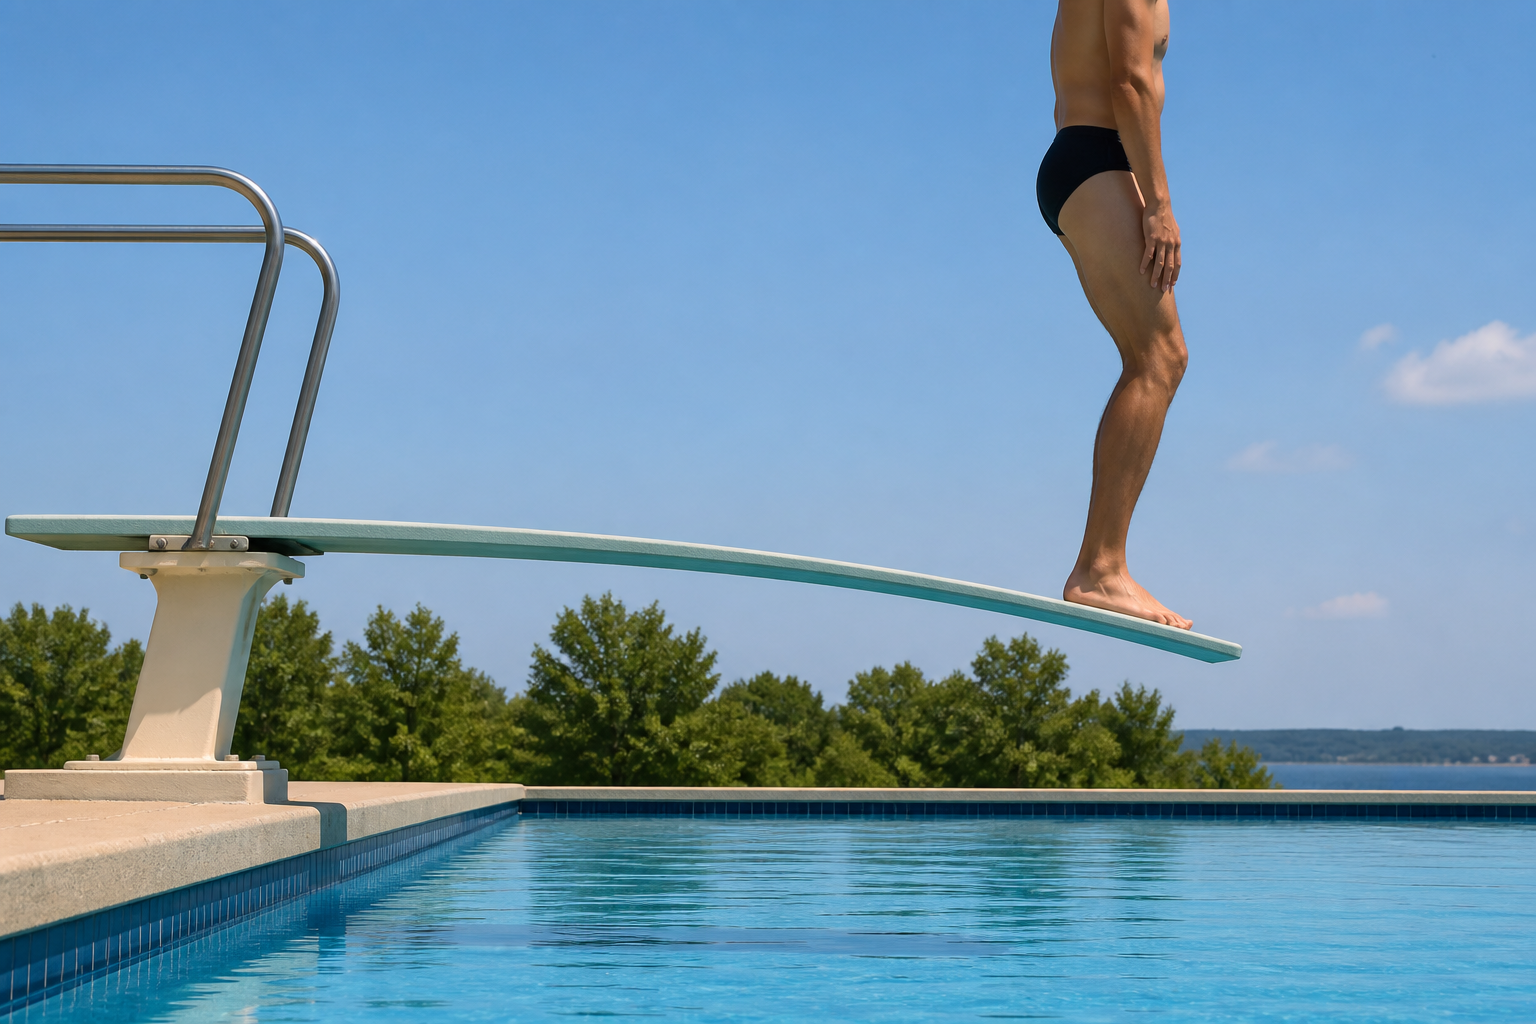
\includegraphics[width=0.58\linewidth]{images/book5/ai/b5-03-diving-board.png}

{\small Un trampolín cargado: tensiones y deformaciones repartidas por un medio continuo, doblado según el perfil cúbico de flexión de la ménsula --- y un resorte a punto de devolver su \omterm{prop:b3:continuum-elasticity:energy}{energía elástica}.}
\end{omfigure}

\section{Ejercicios}

\begin{exercise}[$\star$]\label{exo:b3:continuum-elasticity:1}
(a) Compruébense las unidades: ¿qué es un pascal en términos de kg, m y s, y
cuál es la unidad de la deformación? (b) Un cable de acero trabaja a $\sigma =
\qty{200}{MPa}$: calcúlese su deformación. (c) Una goma elástica ($E \approx
\qty{2}{MPa}$) se estira hasta el doble de su longitud: ¿qué
``deformación'' es esa y por qué no se aplica realmente el marco de este
capítulo? (d) Ordénese por densidad de \omterm{prop:b3:continuum-elasticity:energy}{energía elástica} almacenada a su
tensión de trabajo: el acero a \qty{200}{MPa} y el caucho a \qty{1}{MPa}.
\end{exercise}

\begin{exercise}[$\star$]\label{exo:b3:continuum-elasticity:2}
Calcúlese el \omterm{def:b3:continuum-elasticity:strain}{tensor de deformaciones} de cada \omterm{def:b3:continuum-elasticity:strain}{campo de desplazamientos} y
descríbase la deformación: (a) $\vect u = \alpha(x, y, z)$; (b) $\vect u =
(\gamma y, 0, 0)$; (c) $\vect u = (-\omega y, \omega x, 0)$; (d)
$\vect u = (\varepsilon x, -\nu\varepsilon y, -\nu\varepsilon z)$ ---
¿qué experimento lo realiza?
\end{exercise}

\begin{exercise}[$\star$]\label{exo:b3:continuum-elasticity:3}
La base de una columna de granito de altura $h$ soporta la tensión $\sigma
= \rho gh$. (a) Dedúzcase de la ecuación de equilibrio con gravedad.
(b) El granito se aplasta hacia los \qty{200}{MPa}: ¿cuál es la columna más
alta posible? (c) El Everest tiene \qty{8.8}{km} de altura: coméntese. (d) ¿Por
qué puede una montaña ser algo más alta que una columna de su propia roca
(piénsese en la forma)?
\end{exercise}

\begin{exercise}[$\star$]\label{exo:b3:continuum-elasticity:4}
Una barra de acero ($E = \qty{200}{GPa}$, $\nu = 0.30$) se estira hasta
$\varepsilon = \num{e-3}$. (a) ¿Deformación lateral? (b) ¿Variación
relativa de volumen? (c) ¿Para qué $\nu$ no cambiaría el volumen en
absoluto, y qué material corriente se le acerca? (d) ¿Por qué es imposible
$\nu > 1/2$ (considérese una compresión hidrostática)?
\end{exercise}

\begin{exercise}[$\star\star$]\label{exo:b3:continuum-elasticity:5}
Tensión circunferencial. Un cilindro de pared delgada (radio $R$, espesor
de pared $t \ll
R$) contiene una presión $p$. (a) Equilibrando las fuerzas sobre un
semicilindro de longitud unidad, muéstrese que la pared soporta la tensión
tangencial $\sigma_\theta = pR/t$. (b) Muéstrese que la tensión longitudinal
(equilibrio sobre una sección recta) vale $pR/2t$: un cilindro está
tensionado el doble en dirección circunferencial que a lo largo --- ¿por
dónde se abren las salchichas? (c) Una botella de buceo: $p =
\qty{200}{bar}$, $R = \qty{9}{cm}$, $t = \qty{5}{mm}$: calcúlense
$\sigma_\theta$ y compárese con un límite de fluencia del acero de
\qty{700}{MPa}. (d) ¿Por qué tienen los depósitos de alta presión fondos
hemisféricos?
\end{exercise}

\begin{exercise}[$\star\star$]\label{exo:b3:continuum-elasticity:6}
Un bloque de caucho ($E = \qty{3.0}{MPa}$, $\nu \approx 0.5$), de base $10
\times \qty{10}{cm}$ y altura \qty{2}{cm}, está pegado entre dos placas;
la placa superior se empuja lateralmente con \qty{150}{N}. (a) Calcúlese $G$.
(b) La tensión cortante y el ángulo de cizalladura $\gamma = \sigma_{xy}/G$;
el desplazamiento lateral de la placa superior. (c) ¿Por qué vale
$\nu \approx 1/2$ para el caucho (qué es difícil y qué es fácil para una
maraña de cadenas poliméricas)? (d) Estos bloques de caucho sostienen
edificios enteros en zonas sísmicas: ¿qué propiedad de este apoyo protege al
edificio, su rigidez en compresión o su blandura en cizalladura?
\end{exercise}

\begin{exercise}[$\star\star$]\label{exo:b3:continuum-elasticity:7}
Una cuerda de escalada de longitud $L = \qty{20}{m}$, sección $S =
\qty{80}{mm^2}$ y módulo efectivo $E = \qty{1.2}{GPa}$. (a) Su
rigidez $k = ES/L$. (b) Un escalador de \qty{80}{kg} cae libremente
\qty{4}{m} antes de que la cuerda entre en juego: igualando energías, hállese
el alargamiento máximo de la cuerda (resuélvase la ecuación de segundo grado;
despréciese en una primera pasada la caída que continúa durante el frenado).
(c) Dedúzcanse la fuerza máxima y la deceleración máxima en unidades de $g$.
(d) ¿Por qué debe retirarse una cuerda que ha detenido una caída dura
(adónde fue la energía y qué dice la curva tensión--deformación)?
\end{exercise}

\begin{exercise}[$\star\star$]\label{exo:b3:continuum-elasticity:8}
Torsión. Un hilo de radio $a$, longitud $L$ y módulo de cizalladura $G$ se
retuerce un ángulo $\theta$. (a) Muéstrese que un tubo de radio $r$ situado
en su interior sufre el ángulo de cizalladura $\gamma(r) = r\theta/L$. (b) Su
tensión cortante es $G\gamma$: intégrese $r \times$ tensión sobre la sección
para obtener el par recuperador $\Gamma = (\pi Ga^4/2L)\,\theta$. (c) El
$a^4$: si se reduce el radio a la mitad, ¿en qué factor cae la rigidez de
torsión? (d) Esta blandura extrema es la razón por la que Cavendish (1798)
colgó su balanza de un hilo fino: para $a = \qty{25}{\micro m}$, $L =
\qty{1}{m}$, $G = \qty{40}{GPa}$, calcúlense $C = \pi Ga^4/2L$ y el periodo con
una barra de momento de inercia $I = \qty{5e-4}{kg.m^2}$.
\end{exercise}

\begin{exercise}[$\star\star$]\label{exo:b3:continuum-elasticity:9}
(a) A partir de la deducción con ondas planas de la
\cref{prop:b3:continuum-elasticity:waves}, calcúlense $c_{\text{P}}$ y
$c_{\text{S}}$ para el acero ($E = \qty{200}{GPa}$, $\nu = 0.29$, $\rho =
\qty{7.85e3}{kg/m^3}$). (b) Compárese $c_{\text{P}}$ con la velocidad en
barra delgada $\sqrt{E/\rho}$ y explíquese la diferencia en una frase. (c)
Para el agua ($\mu = 0$, módulo de compresibilidad \qty{2.2}{GPa}): la
velocidad S y la velocidad P. (d) ¿En qué ángulo difiere el movimiento de la
materia de una \omterm{prop:b3:continuum-elasticity:waves}{onda P} del de una \omterm{prop:b3:continuum-elasticity:waves}{onda S}, y cómo las distingue un sismómetro
de tres componentes?
\end{exercise}

\begin{exercise}[$\star\star\star$]\label{exo:b3:continuum-elasticity:10}
Flexión. Una viga se dobla hasta un radio de curvatura $R$; sus fibras
interiores se acortan, las exteriores se alargan y una \emph{superficie
neutra} intermedia conserva su longitud. (a) Muéstrese que la fibra situada
a una distancia $y$ de la superficie neutra tiene deformación
$\varepsilon = y/R$ y, por tanto, tensión $Ey/R$.
(b) Sumando momentos sobre la sección recta, muéstrese que el momento
flector es $M = EI/R$ con $I = \int y^2\,\dd S$ (el \emph{momento de segundo
orden}); calcúlese $I$ para un rectángulo de anchura $b$ y altura $h$. (c) El
$h^3$: ¿por qué un tablón doblado de plano se comba a ojos vistas mientras
el mismo tablón de canto resulta rígido? Calcúlese la razón para $b/h = 5$.
(d) Para una ménsula de longitud $L$ cargada con $F$ en su extremo, la
flecha es $\delta = FL^3/3EI$ (admitido): estímese $\delta$ para un trampolín
($L = \qty{1.8}{m}$, $b = \qty{50}{cm}$, $h = \qty{3.5}{cm}$, madera de $E
= \qty{12}{GPa}$) bajo un saltador de \qty{75}{kg}, y coméntese.
\end{exercise}

\begin{exercise}[$\star\star\star$]\label{exo:b3:continuum-elasticity:11}
Pandeo. Una columna esbelta (longitud $L$, rigidez a flexión $EI$),
articulada en ambos extremos, soporta una carga axial $P$. Supóngase que se
arquea lateralmente según $y(x)$. (a) Muéstrese que la carga ejerce entonces
el momento flector $M(x) = -Py(x)$ respecto del eje desplazado, de modo que
$EI\,y'' = -Py$. (b) Con $y(0) = y(L) = 0$, muéstrese que un arqueo no nulo
se hace posible por primera vez en la carga crítica de Euler
$P_{\text{c}} = \pi^2EI/L^2$. (c) Calcúlese $P_{\text{c}}$ para una regla de
un metro ($b = \qty{3}{cm}$, $h = \qty{1.5}{mm}$, $E = \qty{12}{GPa}$) y
compárese con el empuje de su mano. (d) Explíquese a partir de $I$ por qué los
huesos, el bambú y los cuadros de bicicleta son \emph{tubos}.
\end{exercise}

\begin{exercise}[$\star\star\star$]\label{exo:b3:continuum-elasticity:12}
La velocidad del sonido en un sólido, a partir de los átomos. Modelícese un
sólido como cadenas de átomos de separación $a$ unidos por ``resortes'' de
rigidez $\kappa$; masa atómica $m$. (a) Muéstrese que estirar la cadena se
corresponde con la tracción del medio continuo con $E = \kappa/a$ (cuéntense
resortes por unidad de área y alargamiento por resorte). (b) Muéstrese que
$\rho = m/a^3$ y conclúyase que $c =
\sqrt{E/\rho} = a\sqrt{\kappa/m}$. (c) Estímese $\kappa$ a partir de la
profundidad de un enlace interatómico ($\sim\qty{3}{eV}$ sobre $\sim
\qty{0.1}{nm}$): $\kappa \sim \qty{50}{N/m}$; con $a =
\qty{2.5e-10}{m}$ y $m = \qty{1e-25}{kg}$, estímese $c$. (d) Compárese con
las velocidades del sonido medidas en metales y conclúyase de qué está hecha
la elasticidad cotidiana.
\end{exercise}

\section{Problema: escuchar la Tierra}

\begin{problem}[{Problema de fin de semana --- cómo revelaron los
terremotos el núcleo líquido}]\label{pb:b3:continuum-elasticity:1}
Un solo terremoto hace sonar el planeta entero, y las dos \omterm{prop:b3:continuum-elasticity:waves}{ondas elásticas}
de este capítulo, al atravesarlo, lo radiografían. Este problema sigue la
física desde la \omterm{thm:b3:continuum-elasticity:hooke}{ley de Hooke} en el granito hasta el descubrimiento por
Oldham, en 1906, de que la Tierra tiene un núcleo --- con la estimación de
su tamaño mediante rayos rectos. Tómese para la roca de la corteza y el manto
$E = \qty{75}{GPa}$, $\nu = 1/4$, $\rho = \qty{2.7e3}{kg/m^3}$; radio
terrestre $R_{\text{E}} =
\qty{6371}{km}$.

\medskip\noindent\textbf{Parte I --- La roca como sólido elástico.}
\begin{enumerate}
  \item Calcúlense los coeficientes de Lamé $\mu$ y $\lambda$ de esta
        roca y obsérvese que $\nu = 1/4$ los hace iguales.
  \item Calcúlense $c_{\text{P}}$ y $c_{\text{S}}$, y verifíquese que
        $c_{\text{P}} = \sqrt3\,c_{\text{S}}$.
  \item Un terremoto desliza dos caras de roca varios metros en unos
        segundos: estímese la deformación liberada si un deslizamiento de
        \qty{2}{m} relaja la roca a lo largo de una escala de
        \qty{50}{km}, y la tensión que se había acumulado.
  \item A partir de la densidad de energía $w = \tfrac12 E\varepsilon^2$,
        estímese la \omterm{prop:b3:continuum-elasticity:energy}{energía elástica} por metro cúbico y luego la energía
        contenida en un volumen de $50 \times 50 \times \qty{20}{km^3}$;
        compárese con un megatón (\qty{4.2e15}{J}).
  \item ¿Por qué sacude la \omterm{prop:b3:continuum-elasticity:waves}{onda S} los edificios con más fuerza que la
        \omterm{prop:b3:continuum-elasticity:waves}{onda P} (piénsese en la dirección del movimiento del suelo para una
        onda que llega desde abajo)?
  \item ¿En cuál de las dos ondas cambia de volumen el terreno?
\end{enumerate}

\medskip\noindent\textbf{Parte II --- Las dos llegadas del sismómetro.}
\begin{enumerate}[resume]
  \item Una estación registra la llegada de la P y, un tiempo $\Delta t$
        después, la de la S. Para un foco a distancia $d$ (bastante
        corta como para admitir rayos rectos), muéstrese que
        \[
        d = \frac{\Delta t}{\dfrac{1}{c_{\text{S}}} -
        \dfrac{1}{c_{\text{P}}}} .
        \]
  \item Evalúese el coeficiente: ¿cuántos kilómetros por segundo de
        retardo S--P?
  \item Una estación mide $\Delta t = \qty{28}{s}$: ¿a qué distancia
        está el terremoto?
  \item Una sola estación da una distancia, no un lugar: ¿cuántas
        estaciones determinan el epicentro y cómo, geométricamente?
  \item Las sirenas de alerta temprana de Japón suenan segundos antes
        del temblor fuerte: para un seísmo a \qty{80}{km} bajo una
        ciudad, ¿cuánto aviso proporciona el propio retardo P--S?
  \item Las alertas modernas añaden la velocidad de la luz: la \omterm{prop:b3:continuum-elasticity:waves}{onda P}
        detectada cerca del foco se radia por delante de ambas ondas.
        Para una ciudad situada a \qty{200}{km} del epicentro, ¿cuánto
        tarda en llegar la \omterm{prop:b3:continuum-elasticity:waves}{onda S} tras la ruptura, y qué aviso puede
        dar un mensaje de radio emitido en la primera llegada de la P a
        \qty{20}{km} del foco?
\end{enumerate}

\medskip\noindent\textbf{Parte III --- Ondas que cruzan el planeta.}
\begin{enumerate}[resume]
  \item A las presiones del manto profundo los módulos crecen: las
        velocidades P alcanzan \qty{13.7}{km/s} en la base del manto.
        Tomando una media aproximada $c_{\text{P}} \approx \qty{10}{km/s}$,
        ¿cuánto tarda una \omterm{prop:b3:continuum-elasticity:waves}{onda P} en cruzar la Tierra por un diámetro?
  \item Las estaciones registran seísmos del otro lado del globo: ¿qué
        dice la mera existencia de esas llegadas sobre la Tierra
        profunda (¿es elástica?, ¿está fundida de parte a parte?)?
  \item Defínase el ángulo epicentral $\Delta$ (ángulo en el centro de la
        Tierra entre el foco y la estación). Para rayos rectos,
        muéstrese que la longitud de la cuerda es
        $2R_{\text{E}}\sin(\Delta/2)$.
  \item Evalúense la cuerda y su tiempo de recorrido con rayos rectos para
        $\Delta = 60^\circ$ a la velocidad media $c_{\text{P}} \approx
        \qty{10}{km/s}$.
  \item Hacia 1900, Oldham advirtió que las \omterm{prop:b3:continuum-elasticity:waves}{ondas S} se registran hasta
        $\Delta \approx 103^\circ$ y luego \emph{desaparecen}: no hay
        S directa más allá. ¿Qué propiedad de una región profunda del
        interior terrestre mata las \omterm{prop:b3:continuum-elasticity:waves}{ondas S}, y qué estado de la materia
        tiene esa propiedad?
  \item Las \omterm{prop:b3:continuum-elasticity:waves}{ondas P} más allá de $103^\circ$ no faltan, pero se
        debilitan, se retrasan y se desplazan (una ``zona de sombra''
        hasta $\approx 142^\circ$): ¿por qué una región líquida retrasa
        y refracta las \omterm{prop:b3:continuum-elasticity:waves}{ondas P} sin detenerlas?
  \item Conclúyase en una frase qué hay en el centro de la Tierra.
\end{enumerate}

\medskip\noindent\textbf{Parte IV --- Pesar el núcleo con una regla.}
\begin{enumerate}[resume]
  \item Un rayo S recto que sale del foco roza el núcleo si su máxima
        aproximación al centro iguala el radio del núcleo
        $R_{\text{c}}$. Muéstrese que ese rayo rasante alcanza la
        superficie con el ángulo epicentral $\Delta^* =
        2\arccos(R_{\text{c}}/R_{\text{E}})$.
  \item A partir de $\Delta^* = 103^\circ$, calcúlese $R_{\text{c}}$.
  \item El valor moderno es \qty{3480}{km}: calcúlese su error y explíquese
        su \emph{signo}: los rayos reales se curvan de vuelta hacia la
        superficie a medida que la velocidad crece con la profundidad
        --- arguméntese si los rayos rectos sobrestiman o subestiman el
        núcleo.
  \item En 1936 Inge Lehmann halló llegadas P débiles \emph{dentro} de
        la zona de sombra: ¿qué concluyó que había dentro del núcleo
        líquido?
  \item El radio del núcleo interno es de \qty{1220}{km} y es sólido:
        propóngase la observación de ondas que podría confirmar esa
        solidez (¿qué onda existe allí que el núcleo externo prohíbe?).
  \item Resúmase el resultado con nombre propio: dos velocidades de onda
        elástica en la roca ($5.8$ y \qty{3.3}{km/s}), una onda ausente
        más allá de $103^\circ$ y una regla dan un núcleo líquido de
        radio $\approx \qty{4000}{km}$ --- dentro de un $15\%$ de los
        \qty{3480}{km} modernos, medidos a través de \qty{6000}{km} de
        roca sólida.
\end{enumerate}
\end{problem}
